%%%%%%%%%%%%%%%%%%%%%%%%%%%%%%%%%%%%%%%%%%%%%%%%%%%%%%%%%%%%%%%%%%%%%%%%%%%%
% AGUJournalTemplate.tex: this template file is for articles formatted with LaTeX
%
% This file includes commands and instructions
% given in the order necessary to produce a final output that will
% satisfy AGU requirements, including customized APA reference formatting.
%
% You may copy this file and give it your
% article name, and enter your text.
%
% guidelines and troubleshooting are here: 

%% To submit your paper:
\documentclass[draft]{agujournal2019}
\usepackage{url} %this package should fix any errors with URLs in refs.
\usepackage{lineno}
\usepackage[inline]{trackchanges} %for better track changes. finalnew option will compile document with changes incorporated.
\usepackage{soul}
\linenumbers
%%%%%%%
% As of 2018 we recommend use of the TrackChanges package to mark revisions.
% The trackchanges package adds five new LaTeX commands:
%
%  \note[editor]{The note}
%  \annote[editor]{Text to annotate}{The note}
%  \add[editor]{Text to add}
%  \remove[editor]{Text to remove}
%  \change[editor]{Text to remove}{Text to add}
%
% complete documentation is here: http://trackchanges.sourceforge.net/
%%%%%%%

\draftfalse

%% Enter journal name below.
%% Choose from this list of Journals:
%
% JGR: Atmospheres
% JGR: Biogeosciences
% JGR: Earth Surface
% JGR: Oceans
% JGR: Planets
% JGR: Solid Earth
% JGR: Space Physics
% Global Biogeochemical Cycles
% Geophysical Research Letters
% Paleoceanography and Paleoclimatology
% Radio Science
% Reviews of Geophysics
% Tectonics
% Space Weather
% Water Resources Research
% Geochemistry, Geophysics, Geosystems
% Journal of Advances in Modeling Earth Systems (JAMES)
% Earth's Future
% Earth and Space Science
% Geohealth
%
% ie, \journalname{Water Resources Research}

%%%%%%%%%%%%%%%%%%%%%%%%%%%%%%%%%%%%%%%%%%%%%%%%%%%%%%%%%%%%%%%%%%%%%
%%%%%%%%%%%%%%%%%%%%%%%       REMOVE THIS %%%%%%%%%%%%%%%%%%%%%%%%%%%
\hfuzz=10000pt
\usepackage{comment}  
%%%%%%%%%%%%%%%%%%%%%%%%%%%%%%%%%%%%%%%%%%%%%%%%%%%%%%%%%%%%%%%%%%%%%
%%%%%%%%%%%%%%%%%%%%%%%%%%%%%%%%%%%%%%%%%%%%%%%%%%%%%%%%%%%%%%%%%%%%s

\journalname{Geophysical Research Letters}

\begin{document}

%%%%%%%%%%%%%%%%%%%%%%%%%%%%%%%%%%%%%%%%%%%%%%%
%  TITLE
%
% (A title should be specific, informative, and brief. Use
% abbreviations only if they are defined in the abstract. Titles that
% start with general keywords then specific terms are optimized in
% searches)
%
%%%%%%%%%%%%%%%%%%%%%%%%%%%%%%%%%%%%%%%%%%%%%%%

% Example: \title{This is a test title}

\title{Amplification of the Aerosol Direct Effect in Declining Global Emissions}

%%%%%%%%%%%%%%%%%%%%%%%%%%%%%%%%%%%%%%%%%%%%%%%
%
%  AUTHORS AND AFFILIATIONS
%
%%%%%%%%%%%%%%%%%%%%%%%%%%%%%%%%%%%%%%%%%%%%%%%

% Authors are individuals who have significantly contributed to the
% research and preparation of the article. Group authors are allowed, if
% each author in the group is separately identified in an appendix.)

% List authors by first name or initial followed by last name and
% separated by commas. Use \affil{} to number affiliations, and
% \thanks{} for author notes.
% Additional author notes should be indicated with \thanks{} (for
% example, for current addresses).

% Example: \authors{A. B. Author\affil{1}\thanks{Current address, Antartica}, B. C. Author\affil{2,3}, and D. E.
% Author\affil{3,4}\thanks{Also funded by Monsanto.}}

\authors{Antoine Hermant\affil{1}, Linnea Huusko\affil{1}, Thorsten Mauritsen\affil{1}}

\affiliation{1}{Department of Meteorology, Stockholm University, Stockholm, Sweden}

% \affiliation{=number=}{=Affiliation Address=}
%(repeat as many times as is necessary)


% Corresponding author mailing address and e-mail address:

% (include name and email addresses of the corresponding author.  More
% than one corresponding author is allowed in this LaTeX file and for
% publication; but only one corresponding author is allowed in our
% editorial system.)

% Example: \correspondingauthor{First and Last Name}{email@address.edu}

\correspondingauthor{Antoine Hermant}{antoine.hermant@misu.su.se}

%%%%%%%%%%%%%%%%%%%%%%%%%%%%%%%%%%%%%%%%%%%%%%%
% KEY POINTS
%%%%%%%%%%%%%%%%%%%%%%%%%%%%%%%%%%%%%%%%%%%%%%%
%  List up to three key points (at least one is required)
%  Key Points summarize the main points and conclusions of the article
%  Each must be 140 characters or fewer with no special characters or punctuation and must be complete sentences

% Example:
% \begin{keypoints}
% \item	List up to three key points (at least one is required)
% \item	Key Points summarize the main points and conclusions of the article
% \item	Each must be 140 characters or fewer with no special characters or punctuation and must be complete sentences
% \end{keypoints}

\begin{keypoints}
\item Global direct effect from anthropogenic aerosols has continued to increase despite declining aerosol emissions. 
\item The shift in aerosol pattern throughout the 1970--2014 period has implication in the continued increase in direct effect.
\item Regional variations in aerosol forcing efficiency are associated with cloudiness, aerosol residence time and surface albedo.
\end{keypoints}

%%%%%%%%%%%%%%%%%%%%%%%%%%%%%%%%%%%%%%%%%%%%%%%
%
%  ABSTRACT and PLAIN LANGUAGE SUMMARY
%
% A good Abstract will begin with a short description of the problem
% being addressed, briefly describe the new data or analyses, then
% briefly states the main conclusion(s) and how they are supported and
% uncertainties.

% The Plain Language Summary should be written for a broad audience,
% including journalists and the science-interested public, that will not have 
% a background in your field.
%
% A Plain Language Summary is required in GRL, JGR: Planets, JGR: Biogeosciences,
% JGR: Oceans, G-Cubed, Reviews of Geophysics, and JAMES.
% see http://sharingscience.agu.org/creating-plain-language-summary/)
%
%%%%%%%%%%%%%%%%%%%%%%%%%%%%%%%%%%%%%%%%%%%%%%%

%% \begin{abstract} starts the second page

\begin{abstract}
Anthropogenic aerosol particles partially mask global warming driven by greenhouse gases, both by directly reflecting sunlight back into space and indirectly by increasing cloud reflectivity, which also results in sunlight reflection. In recent decades, however, the emissions of anthropogenic aerosols have declined globally, and at the same time shifted from the North American and European regions to foremost Southeast Asia. Using global climate model simulations we find that the direct cooling effect of aerosols has instead continued to increase, despite declining emissions, whereas the indirect effect has weakened in approximate proportion with the emissions. The enhanced efficiency of the aerosol direct effect is associated with less cloudiness, longer atmospheric residence time, and emissions over darker surfaces in the Southeast Asian region.
\end{abstract}

\section*{Plain Language Summary}
Enter your Plain Language Summary here or delete this section.
%Here are instructions on writing a Plain Language Summary: 
%https://www.agu.org/Share-and-Advocate/Share/Community/Plain-language-summary


%%%%%%%%%%%%%%%%%%%%%%%%%%%%%%%%%%%%%%%%%%%%%%%
%
%  BODY TEXT
%
%%%%%%%%%%%%%%%%%%%%%%%%%%%%%%%%%%%%%%%%%%%%%%%

%%% Suggested section heads:
% \section{Introduction}
%
% The main text should start with an introduction. Except for short
% manuscripts (such as comments and replies), the text should be divided
% into sections, each with its own heading.

% Headings should be sentence fragments and do not begin with a
% lowercase letter or number. Examples of good headings are:

% \section{Materials and Methods}
% Here is text on Materials and Methods.
%
% \subsection{A descriptive heading about methods}
% More about Methods.
%
% \section{Data} (Or section title might be a descriptive heading about data)
%
% \section{Results} (Or section title might be a descriptive heading about the
% results)
%
% \section{Conclusions}


\section{Introduction}
      Global climate models participating in the Coupled Model Intercomparison Project phase 6 (CMIP6) predict a high climate sensitivity \cite{Flynn_2020}. However, the majority of models simulate a reduced historical warming, with global temperatures systematically colder than observations from 1940 to 2000. The proposed explanation for this discrepancy lies in the rapid increase in atmospheric aerosols, with the belief that models use a strong aerosol cooling effect to compensate for their high sensitivity. Moreover, it is thought that the implementation of air quality regulations since the 1970s has stabilized this effect, allowing the models to align with observations in the early 21st century \cite{Flynn_2020}. 

      They are a significant source of uncertainty in climate models due particularly to their complex interactions with clouds \cite{Bellouin_2020}. 
      In addition to the reduction in global emissions, aerosols have change in emission pattern. Previous studies looked at the shift in pattern does not affect the aerosol forcing. 
      Here we used a novel approach for assessing the anthropogenic aerosol forcing in CMIP6 which allows use to more accurately investigate the emission spatial pattern on aerosol forcing. 

\section{Method}\label{sec:method}
      We study the historical evolution of the aerosol forcing using the Max Planck Institute for Meteorology Earth System Model version 1.2. MPI-ESM1.2, a state-of-the-art climate model \cite{Mauritsen_2019} that participated in the Coupled Model Intercomparison Project Phase 6 (CMIP6), successfully reproduces the observed warming from pre-industrial levels \cite{Mauritsen_2020}.
      The radiative transfer scheme of MPI-ESM1.2 uses the simple plume implementation of the second version of the Max Planck Institute Aerosol Climatology (MACv2-SP) to represent the aerosol impact on the radiation. MACv2-SP provides a parametrization of optical properties of anthropogenic aerosols and the resulting Twomey effect \cite{Stevens_2017}. It has been designed with the desire of an uniform and easily controlled representation of anthropogenic aerosol perturbations for the CMIP6 framework \cite{Pincus_2016}. To achieve this, \citeA{Stevens_2017} constructed nine spatial plumes that are associated with emissions from major anthropogenic source regions. They used aerosol optical properties estimates from ground-based measurements provided by the Max Planck Institute Aerosol Climatology, MAC \cite{Kinne_2013}, for the present-day (2005) distribution of mid-visible anthropogenic aerosol optical depth. Then, past changes are represented scaling the obtained present-day distribution with the historical emissions of source regions, estimates of the Community Emissions Data System (CEDS) for the period spanning from pre-industrial (1850) to 2016. Two types of plumes are considered: industrial (Europe, North America, Australia, East and South Asia) and biomass burning (South America, Maritime Continental, North and South Central Africa), where they differ in seasonal cycle amplitude, single-scattering albedo and strength in Twomey effect. 
      MACv2-SP also provides a parametrisation of the Twomey effect accounting for aerosol-cloud interactions. \citeA{Stevens_2017} used satellite observations to derive the relationship between the cloud droplet number density $N$ and the fine-mode AOD. This way, anthropogenic aerosols cause a greater increase in cloud albedo when the cloud is originally optically thin, or in other terms, when the environment is originally pristine from aerosols.
      For the full description of MACv2-SP, refer to \citeA{Stevens_2017}.

      Since MPI-ESM1.2 uses an offline radiative transfer scheme (cite), the Partial Radiative Perturbation (PRP) method can be performed and has been implemented by \citeA{Meraner_2013}. The PRP method has been first described by \citeA{Wetherald_1988} and aims to determine the influence of the individual climate feedbacks on the TOA radiative imbalance. In our work, we developed the existing PRP module in MPI-ESM1.2 for allowing to perform in historical simulations and extend the diagnostic to anthropogenic aerosols.
      As the PRP method has been designed to isolate the contribution from the climate feedbacks to the TOA radiative imbalance, our method distinguishes from other method to calculate aerosol forcing by solely isolating aerosol contribution to the radiative imbalance. The PRP can then be used in fully-coupled model standard historical simulations. In the radiative transfer scheme of MPI-ESM1.2, both direct and indirect effects of anthropogenic aerosols are represented separately as distinct perturbations in the climate system. This separation enables us to assess the contribution to the radiative imbalance from each effect individually by substituting them one at a time into the PRP method. Thus, the PRP allows to accurately separate the forcing from the direct and indirect effects of anthropogenic aerosols. More details on our PRP approach and its application to anthropogenic aerosols can be found in the Supplement.
      
\begin{comment}
      The Partial Radiative Perturbation method has been first described by \citeA{Wetherald_1988} and aims to determine the influence of the individual climate feedbacks (\ref{eq:sum-lambda}) on the TOA radiative imbalance (\ref{eq:linear}). It is based on recomputing radiative fluxes for changed states which is computationally expensive and requires a decoupled radiative transfer scheme from the model. The implementation of the method in ECHAM was carried out by \cite{Meraner_2013}. The present work consists in developing the existing module to diagnostic aerosol forcing on the TOA radiative imbalance.

      When introducing a radiative forcing in the climate system at stable state ($\delta R = 0$), the individual climate feedbacks will respond and add or remove some radiative forcing. The total radiative forcing at TOA can then be written:
      \begin{equation}\label{eq:sum-R}
            \delta R = \delta_z R + \delta_{plk} R + \delta_{lr} R + \delta_{vap} R + \delta_{alb} R + \delta_{cld} R,
      \end{equation}
      where $\delta_z R$ is the contribution of an applied perturbation. \citeA{Wetherald_1988} points out that the perturbation should be sufficiently small to fullfil the linear approach and hold Eq. \ref{eq:sum-R}. With this approach, the TOA radiation fluxes can be recalculated by substituting one at a time the fields from a perturbed climate while taking all other fields from a control state. The partial perturbations are then obtained by subtracting the control TOA net radiation flux to the recomputed fluxes. However, interactions between feedbacks are neglected and that the difference between the perturbed and the control state must be small enough to hold the discrete approximation of the derivative by the differentiation \cite{Wetherald_1988}.

      Assuming linearity, the perturbation to get from the control state to the perturbed state (forward) should be equal to the perturbation to get back to the control state from the perturbed state (backward), but with opposite sign. However, the perturbation is sensitive to the state in which it is introduced \cite{Colman_1997} and de-correlating variables when substituting fields introduces unintended perturbations \cite{Klocke_2013}. The proposed method to partially overcome these approximations is to apply the partial radiative perturbation forward ($\delta_{z} R^{FW}$) and backward ($\delta_{z} R^{BW}$), and to take the mean of the obtained fluxes \cite{Klocke_2013}. For a small perturbation $\delta z$, 
      \begin{equation}\label{eq:fw}
          \delta_{z} R^{FW} = R(z + \delta z, plk, lr, alb, cld) - R(z, plk, lr, alb, cld),
      \end{equation}
      \begin{equation}\label{eq:bw}
          \delta_{z} R^{BW} = R(z, plk', lr', alb', cld') - R(z + \delta z, plk', lr', alb', cld'),
      \end{equation}
      and the final approximation:
      \begin{equation}
          \delta_{z} R = \frac{\delta_{z} R^{FW} - \delta_{z} R^{BW}}{2}.
      \end{equation}

      The PRP method was originally designed to quantify the individual feedbacks within the climate system. However, at its core, the method calculates the forcing resulting from a perturbation. It is based on this fundamental characteristic that the present study proposes to utilize the PRP method to quantify the forcing induced by anthropogenic aerosols. By applying the PRP method to aerosol perturbations, it allows for the assessment and quantification of the forcing induced by aerosols in the climate system.

      In this work, the perturbation in Equations \ref{eq:fw} and \ref{eq:bw} is aerosols, with $z$ the background aerosols and $\delta z$ is the implementation of anthropogenic aerosols. Additionally, the perturbation from anthropogenic aerosols can be separated into the forcing from direct and indirect effect. As seen in the previous Section, the indirect effect takes the form of an empirical equation (Eq. \ref{eq:twomey}) for the cloud droplet number density, considering the background AOD and anthropogenic AOD. Thus, we can calculate the forcing from the direct effect by substituting into the control the AOD from the anthropogenic aerosol but fixing the cloud droplet to the background level $N_{1850}$ and vice versa into the perturbed state. The forcing from the indirect effect is obtained by substituting into the control state the perturbed cloud droplet number density $N$ but fixing the AOD to the background level and vice versa into the perturbed state.

\end{comment}


\section{Results}

      \subsection{Historical Aerosol Forcing}
            Our PRP diagnostic, which assesses anthropogenic aerosol forcing in historical simulations, reveals a consistent and increasing cooling effect from aerosols, despite the global reduction in their emissions (see Fig. \ref{fig:global-forcing}). This persistent cooling trend is primarily driven by the direct effect, which continues to increase even after the implementation of regulations in Europe and North America since the 1980s. Meanwhile, the indirect effect diminishes in approximate proportion to decreasing emissions.
            In addition to the global decrease in aerosol emissions, the period spanning from 1980 to 2005 witnessed a shift in aerosol patterns. Aerosol concentrations transitioned from being primarily centered in Europe and North America to becoming more concentrated in Southern and Eastern Asian regions.
            The subsequent sections investigate the role played by this geographical shift in explaining the observed discrepancy between aerosol emissions and their associated forcing.

      \begin{figure}
            \centering
            \noindent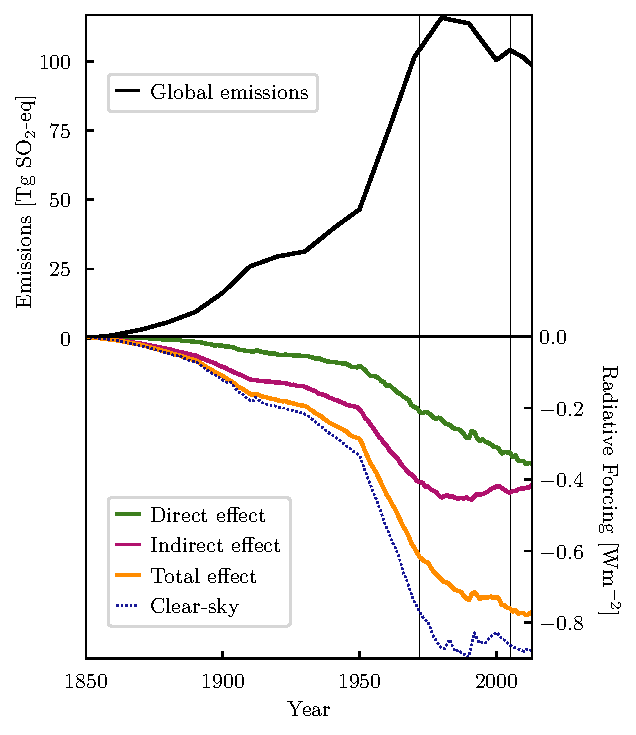
\includegraphics[width=0.5\textwidth]{../../figures/figure1}
            \caption{Historical anthropogenic aerosol emissions and their associated radiative forcing. Values are global yearly means. Vertical lines indicate the years 1972 and 2005 when emission levels were identical but led to different total aerosol forcing.}
            \label{fig:global-forcing}
      \end{figure}

      \subsection{Forcing from Regional Aerosol Sources}
            As detailed in Section \ref{sec:method}, MACv2-SP provided a parametrisation for anthropogenic aerosols, incorporating nine distinct simple-plumes that represent various anthropogenic emission regions. To assess the aerosol forcing from each of these regions, we substituted one plume at a time into the PRP (see Sec. \ref{sec:method}). Fig. \ref{fig:individual-plumes} illustrates the resulting forcing values from each region plotted against their respective aerosol emissions (in [Tg SO$_2$]$_{eq}$). In Fig. \ref{fig:individual-plumes}.a., we observe a significant variability in emission efficiency of the direct effect among major industrial regions, such as Europe, North America, East and South Asia, and Australia. Notably, South Asia exhibits an efficiency 20.10 times greater than Europe, representing the most substantial difference in efficiency across these regions. On the other hand, Fig. \ref{fig:individual-plumes}.b. shows a relatively more consistent relationship between forcing and emissions for the indirect effect across regions. 
            The regional variation in efficiency explains the persistent increase in the global direct effect. Regions with higher efficiency have a more substantial impact on the global direct effect while emitting fewer aerosols. This effect becomes particularly evident when considering the shift in aerosol patterns from 1980 to 2005. During this period, aerosol emissions shifted from Europe and North America to Southeast Asia, where higher emission efficiencies prevailed. Consequently, despite reduced global emissions during this timeframe, the global aerosol forcing continued to rise.
            Subsequent sections delve into the mechanisms that underlie these regional variations in aerosol emission efficiency.

      \begin{figure}
            \centering
            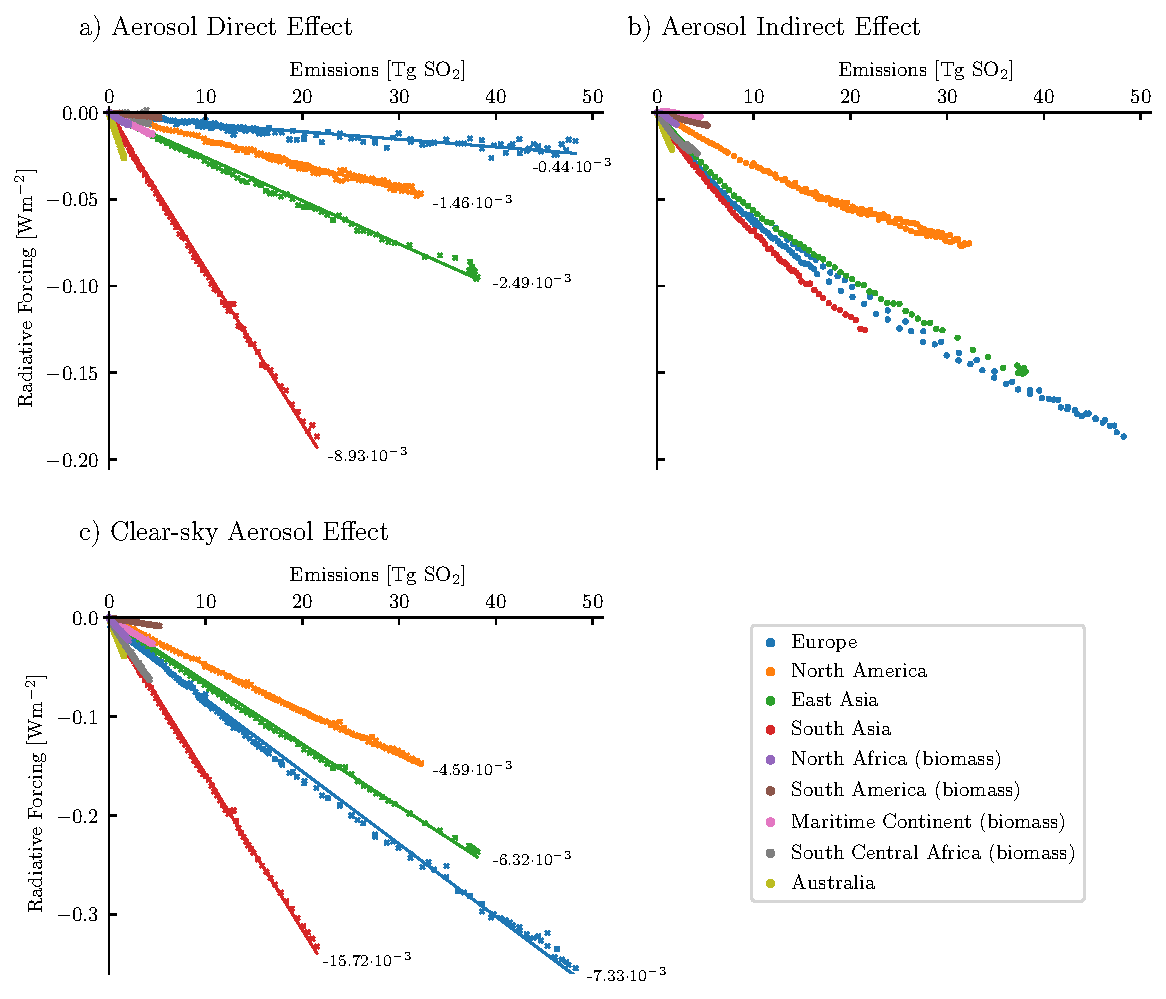
\includegraphics[width=\textwidth]{../../figures/figure2}
            \caption{Forcing from the direct and indirect aerosol effects against emissions for individual emission regions as global yearly means. Values on the plots are the emission efficiencies (in Wm$^{-2}$ per Tg of $_{eq}$SO$_2$) for the major regions, based on linear regression.}
      \label{fig:individual-plumes}
      \end{figure}

      \subsection{All-sky vs Clear-sky Aerosol Forcing}
            We examine the outcomes of the PRP performed under both all-sky and clear-sky conditions. The results of all-sky conditions, separated into direct and indirect effects, confirms the predominant occurrence of the direct effect in the vicinity of emission sources (see Fig. \ref{fig:maps}.c.). Conversely, the indirect effect, which is larger than the direct effect, occurs predominantly over remote regions, particularly over oceans (see Fig. \ref{fig:maps}.b.), aligning with the findings of \citeA{Huusko_2022}.
            The global clear-sky aerosol forcing surpasses the global total forcing (direct + indirect effects) observed in all-sky conditions (see Fig. \ref{fig:global-forcing}), despite the only occurrence the direct effect in clear-sky conditions. Notably, the clear-sky aerosol forcing is more than twice as significant as the direct effect observed in all-sky conditions. This observation holds true across all emission regions, with clear-sky aerosol forcing consistently exceeding the direct effect (see Fig \ref{fig:individual-plumes}.a. and c.). 
            Under all-sky conditions, the presence of extensive cloud cover results in a neutral or positive forcing from the direct effect of aerosols (see Fig. \ref{fig:maps}.c. and e.). Specifically, in regions characterized by high cloud reflectivity in their natural state, anthropogenic aerosol emissions atop the clouds contribute to the net absorption of shortwave radiation. In regions with robust cloud systems, the negative forcing arising from the indirect effect through clouds and the positive direct effect tend to balance each other, resulting in nearly zero total aerosol effect (see Fig. \ref{fig:maps}.a. and e.)
            This mechanism has significant implications for regional emission efficiency. In particular, it explains why Europe, which exhibits weak emission efficiency under all-sky (Fig. \ref{fig:individual-plumes}.a.) due to warming direct effect at high latitudes (Fig. \ref{fig:maps}), demonstrates greater efficiency under clear-sky conditions. Looking at clear-sky conditions significantly narrows the gap in regional efficiencies. The ratio between South Asia and Europe decreases to 2.1 in clear-sky (compared to 20.1 for the all-sky direct effect), and the most substantial difference emerges between South Asia and North America, with a efficiency ratio of 3.2.
            The interaction between cloud cover and the direct effect of anthropogenic aerosols emerges as a main factor influencing regional emission efficiency. This largely explains the consistent increase in aerosol cooling despite reduced emissions. As Southeast Asian regions present less cloud cover at the emission sources compared to Europe, the shift in aerosol patterns results in enhanced global direct effect. The presence of clouds in remote regions, stemming from Southeast Asian sources, such as over the Indian and Pacific Oceans, maintains the significance of the indirect effect despite the pattern shift. Overall, emission efficiency in greater in Southeast Asian regions compared to Europe and North America.
            The resulting increase in emission efficiency from the shift in aerosol pattern is critical in the enhanced aerosol forcing observed when comparing the mid-1970s to the mid-2000s, even though emissions levels were similar.
            However, the disparity in emission efficiencies among regions remains substantial under clear-sky conditions. The following sections investigate the factors contributing to these regional differences.
            
      \begin{figure}
            \centering
            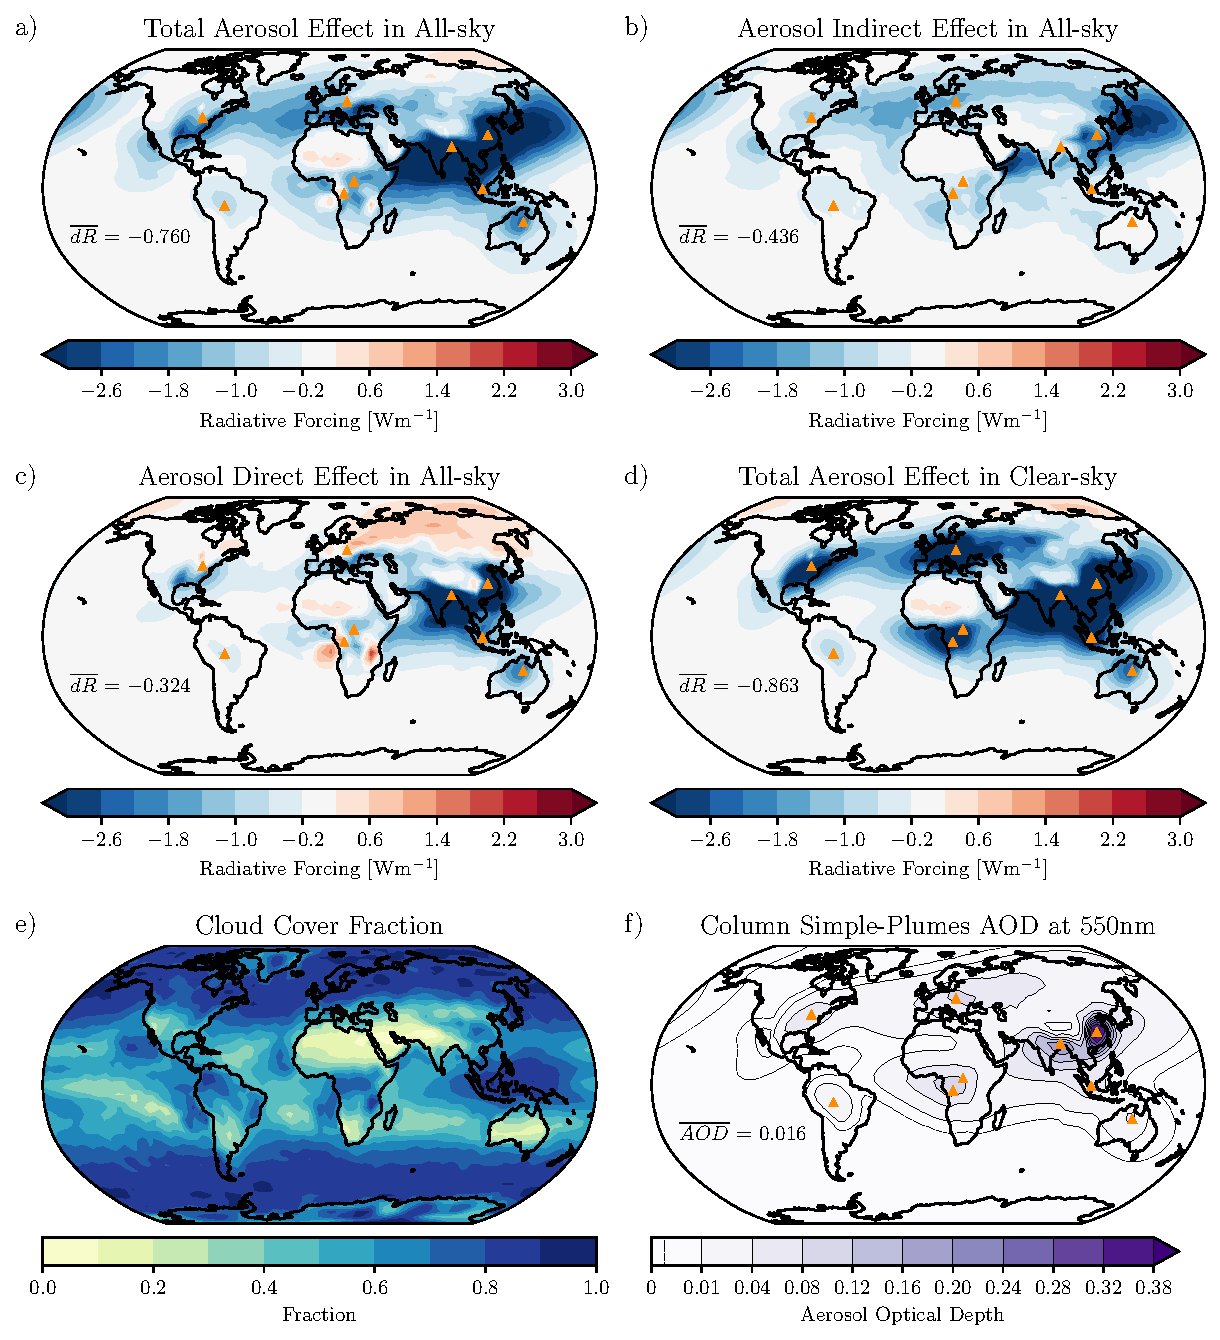
\includegraphics[width=0.9\textwidth]{../../figures/figure3}
            \caption{Anthropogenic aerosol forcing in the 2005-aerosol pattern, and associated cloud cover and AOD patterns. Values on the maps are global means. In f), dashed-line shows low AOD value contour (0.0025) provided by the MACv2-SP parametrisation.}
            \label{fig:maps}
      \end{figure}

      \subsection{Aerosol Removal Processes}
            The MACv2-SP has been designed to simplify the representation of anthropogenic aerosols in climate models through a straightforward parametrisation. 
            It provides monthly mean Aerosol Optical Depth (AOD) from the ground-based measured 2005 distribution that have been scaled with estimates of historical emissions. 
            Consequently, the AOD in MACv2-SP may not always exhibit a direct proportionality to emissions from various regions due to regional variation in aerosol removal processes.
            Fig. \ref{fig:figure4}.a. shows the clear-sky aerosol forcing plotted against the corresponding AOD levels for each region. This representation significantly reduces the spread in efficiency between regions. For instance, the ratio of efficiencies in Wm$^{-2}$ per unit of AOD between South Asia to Europe stands at 1.3, against 2.1 when in Wm$^{-2}$ per unit of emissions. 
            Interestingly, when considering AOD levels, both Asian regions exhibit similar efficiencies, which contrasts with the scenario when considering emissions. This difference arises because storm tracks over the Pacific Ocean play a significant role in aerosol removal. They effectively remove a substantial amount of aerosols, resulting in lower forcing per unit of emissions for East Asia. Conversely, the relatively stable atmospheric conditions over the Indian Ocean contribute to a higher forcing per unit of emissions for South Asia.
            Similarly, storm tracks over the Atlantic Ocean lead to the efficient removal of aerosols from North America, resulting in a weaker efficiency in forcing relative to emissions. In contrast, aerosols in Europe are transported over longer distances without significant removal, leading to a higher efficiency in forcing relative to emissions in clear-sky conditions.
            This difference in aerosol removal patterns is the second most significant explanation for the continued increase in aerosol forcing despite reduced emissions. The shift in aerosol patterns from Europe and North America towards Southeast Asian regions, with more stable conditions, prolongs the residence time of aerosols in the atmosphere, consequently enhancing the emission efficiency.
            The last section, we suggest additional explanations for the remaining minor differences in emission efficiency between regions.

      \begin{figure}
            \centering
            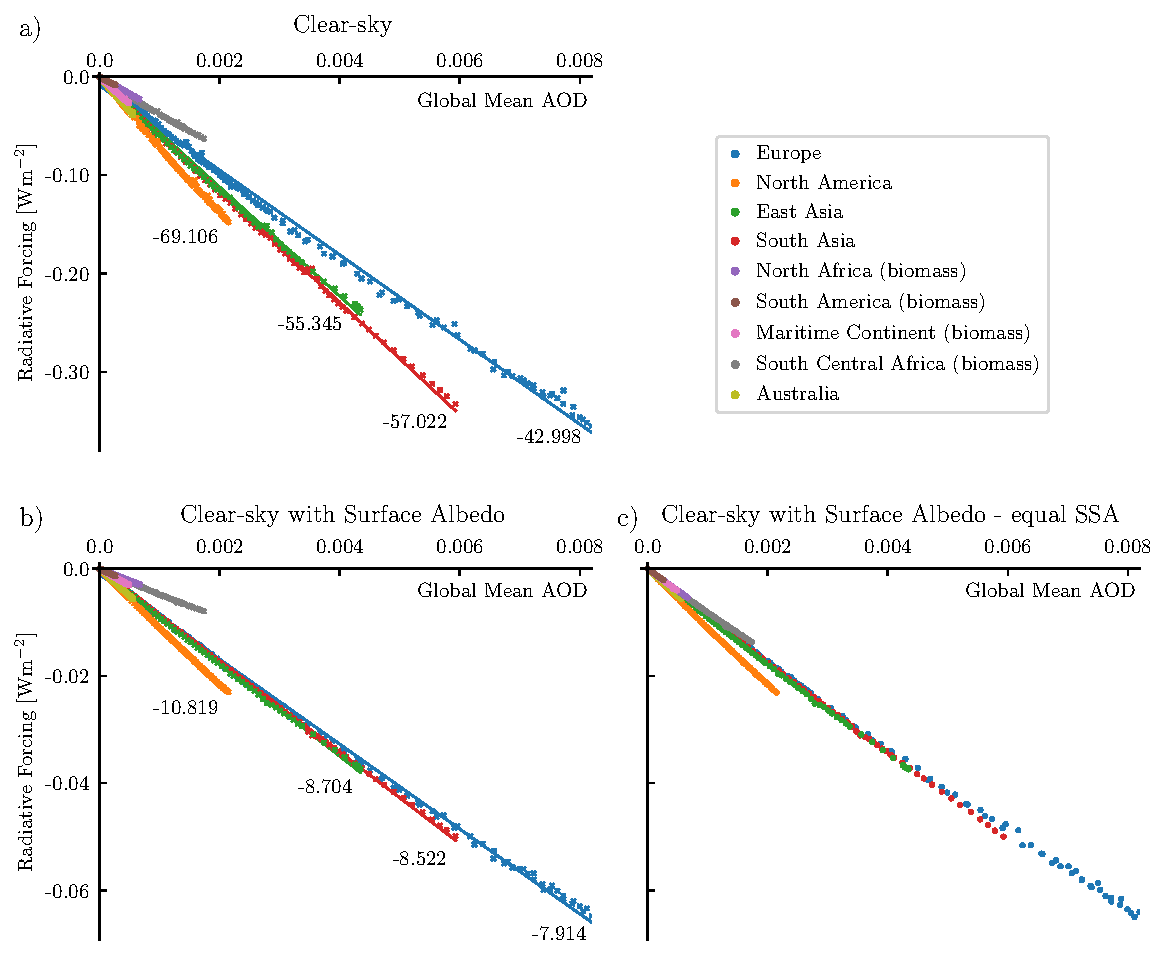
\includegraphics[width=0.9\textwidth]{../../figures/figure4}
            \caption{Clear-sky anthropogenic aerosol forcing plotted against AOD for individual emission regions. Values on the plots are the emission efficiencies (in Wm$^{-2}$ per unit of AOD)for the major regions, based on linear regression. In b), the radiative forcing is adjusted by the surface albedo, while c) replicates b), but with the Single-Scattering Albedo (SSA) is set to the same value for both industrial and biomass aerosol sources.}
            \label{fig:figure4}
      \end{figure}

      \subsection{Surface and Aerosol Single-Scattering Albedo}

            The remaining differences in clear-sky efficiency among industrial regions appear to be closely related to surface albedo (Fig. \ref{fig:figure4}.b.). When multiplied by surface albedo, the ratio of efficiencies in Wm$^{-2}$ per unit of AOD between South Asia and Europe is reduced to 1.08 (against 1.3 without surface albedo adjustments). Just as we discussed in the context of cloud cover in Section [...], anthropogenic aerosol forcing also depends on the nature of the underlying surface. In areas with inherently reflective surfaces, aerosol emissions can contribute to the net absorption of shortwave radiation. This clarifies why Europe, which emits aerosols in high-latitudes over snow-covered and icy regions, exhibits weaker efficiency compared to regions with darker surfaces, such as Asia. It's important to note that this effect is primarily observed in clear-sky forcing, as in all-sky conditions, the direct effect is largely influenced by interactions with cloud reflectivity detailed in Section ..... Nonetheless, these findings suggest that a shift in aerosol patterns towards regions with darker surfaces can lead to greater aerosol forcing for similar emission levels.
            
            Distinguishing between industrial and biomass aerosol emissions hinges primarily on the Single-Scattering Albedo (SSA) parameter provided by MACv2-SP, which is 0.93 for industrial and 0.87 for biomass. This difference explains why the efficiencies of biomass regions remain weaker compared to industrial regions. In Fig. \ref{fig:figure4}.c., we provide an identical representation to Fig. \ref{fig:figure4}.b., but with the SSA of biomass regions set to the same value as for industrial regions, effectively eliminating the disparities.
            It's important to note that this observation holds true in all-sky conditions as well, as SSA defines the ratio of scattering efficiency to total extinction efficiency. However, it plays a relatively minor role in the overall discrepancy, given that biomass regions typically have smaller emissions and smaller forcing. In fact, biomass emissions would actually contribute to a decrease in global emission efficiency if they were more significant, as their SSA value implies greater shortwave absorption.

\section{Discussion and Conclusions}
      

%  Numbered lines in equations:
%  To add line numbers to lines in equations,
%  \begin{linenomath*}
%  \begin{equation}
%  \end{equation}
%  \end{linenomath*}



%% Enter Figures and Tables near as possible to where they are first mentioned:
%
% DO NOT USE \psfrag or \subfigure commands.
%
% Figure captions go below the figure.
% Acronyms used in figure captions will be spelled out in the final, published version.

% Table titles go above tables;  other caption information
%  should be placed in last line of the table, using
% \multicolumn2l{$^a$ This is a table note.}
% NOTE that there is no difference between table caption and table heading in the final, published version
%
%----------------
% EXAMPLE FIGURES
%
% \begin{figure}
% \includegraphics{example.png}
% \caption{caption}
% \end{figure}
%
% Giving latex a width will help it to scale the figure properly. A simple trick is to use \textwidth. Try this if large figures run off the side of the page.
% \begin{figure}
% \noindent\includegraphics[width=\textwidth]{anothersample.png}
%\caption{caption}
%\label{pngfiguresample}
%\end{figure}
%
%
% If you get an error about an unknown bounding box, try specifying the width and height of the figure with the natwidth and natheight options. This is common when trying to add a PDF figure without pdflatex.
% \begin{figure}
% \noindent\includegraphics[natwidth=800px,natheight=600px]{samplefigure.pdf}
%\caption{caption}
%\label{pdffiguresample}
%\end{figure}
%
%
% PDFLatex does not seem to be able to process EPS figures. You may want to try the epstopdf package.
%

%
% ---------------
% EXAMPLE TABLE
%
% \begin{table}
% \caption{Time of the Transition Between Phase 1 and Phase 2$^{a}$}
% \centering
% \begin{tabular}{l c}
% \hline
%  Run  & Time (min)  \\
% \hline
%   $l1$  & 260   \\
%   $l2$  & 300   \\
%   $l3$  & 340   \\
%   $h1$  & 270   \\
%   $h2$  & 250   \\
%   $h3$  & 380   \\
%   $r1$  & 370   \\
%   $r2$  & 390   \\
% \hline
% \multicolumn{2}{l}{$^{a}$Footnote text here.}
% \end{tabular}
% \end{table}

%%%%%%%%%%%%%%%%%%%%%%%%%%%%%%%%%%%%%%%%%%%%%%%
% SIDEWAYS FIGURES and TABLES
% AGU prefers the use of {sidewaystable} over {landscapetable} as it causes fewer problems.
%
% \begin{sidewaysfigure}
% \includegraphics[width=20pc]{figsamp}
% \caption{caption here}
% \label{newfig}
% \end{sidewaysfigure}
%
%  \begin{sidewaystable}
%  \caption{Caption here}
% \label{tab:signif_gap_clos}
%  \begin{tabular}{ccc}
% one&two&three\\
% four&five&six
%  \end{tabular}
%  \end{sidewaystable}

%% If using numbered lines, please surround equations with \begin{linenomath*}...\end{linenomath*}
%\begin{linenomath*}
%\begin{equation}
%y|{f} \sim g(m, \sigma),
%\end{equation}
%\end{linenomath*}

%%% End of body of article

%%%%%%%%%%%%%%%%%%%%%%%%%%%%%%%%%%%%%%%%%%%%%%%
%% Optional Appendices go here
%
% The \appendix command resets counters and redefines section heads
%
% After typing \appendix
%
%\section{Here Is Appendix Title}
% will show
% A: Here Is Appendix Title
%
%\appendix
%\section{Here is a sample appendix}

%%%%%%%%%%%%%%%%%%%%%%%%%%%%%%%%%%%%%%%%%%%%%%%
% Optional Glossary, Notation or Acronym section goes here:
%
% Glossary is only allowed in Reviews of Geophysics
%  \begin{glossary}
%  \term{Term}
%   Term Definition here
%  \term{Term}
%   Term Definition here
%  \term{Term}
%   Term Definition here
%  \end{glossary}


%%%%%%%%%%%%%%%%%%%%%%%%%%%%%%%%%%%%%%%%%%%%%%%
% Acronyms
%% NOTE that acronyms in the final published version will be spelled out when used in figure captions.
%   \begin{acronyms}
%   \acro{Acronym}
%   Definition here
%   \acro{EMOS}
%   Ensemble model output statistics
%   \acro{ECMWF}
%   Centre for Medium-Range Weather Forecasts
%   \end{acronyms}


%%%%%%%%%%%%%%%%%%%%%%%%%%%%%%%%%%%%%%%%%%%%%%%
% Notation
%   \begin{notation}
%   \notation{$a+b$} Notation Definition here
%   \notation{$e=mc^2$}
%   Equation in German-born physicist Albert Einstein's theory of special
%  relativity that showed that the increased relativistic mass ($m$) of a
%  body comes from the energy of motion of the body—that is, its kinetic
%  energy ($E$)—divided by the speed of light squared ($c^2$).
%   \end{notation}




%%%%%%%%%%%%%%%%%%%%%%%%%%%%%%%%%%%%%%%%%%%%%%%
%
% DATA SECTION and ACKNOWLEDGMENTS
%
%%%%%%%%%%%%%%%%%%%%%%%%%%%%%%%%%%%%%%%%%%%%%%%

\section*{Open Research Section}
This section MUST contain a statement that describes where the data supporting the conclusions can be obtained. Data cannot be listed as ''Available from authors'' or stored solely in supporting information. Citations to archived data should be included in your reference list. Wiley will publish it as a separate section on the paper’s page. Examples and complete information are here:
%https://www.agu.org/Publish with AGU/Publish/Author Resources/Data for Authors


\acknowledgments
Enter acknowledgments here. This section is to acknowledge funding, thank colleagues, enter any secondary affiliations, and so on.


%%%%%%%%%%%%%%%%%%%%%%%%%%%%%%%%%%%%%%%%%%%%%%%
% REFERENCES and BIBLIOGRAPHY
%
\bibliography{/home/anthe/documents/misu/paper_aerosols/latex/bibtex/paper_aerosols} 
 %don't specify the file extension
% don't specify bibliographystyle
%
%%%%%%%%%%%%%%%%%%%%%%%%%%%%%%%%%%%%%%%%%%%%%%%

%\bibliography{ enter your bibtex bibliography filename here }



%Reference citation instructions and examples:
%
% Please use ONLY \cite and \citeA for reference citations.
% \cite for parenthetical references
% ...as shown in recent studies (Simpson et al., 2019)
% \citeA for in-text citations
% ...Simpson et al. (2019) have shown...
%
%
%...as shown by \citeA{jskilby}.
%...as shown by \citeA{lewin76}, \citeA{carson86}, \citeA{bartoldy02}, and \citeA{rinaldi03}.
%...has been shown \cite{jskilbye}.
%...has been shown \cite{lewin76,carson86,bartoldy02,rinaldi03}.
%... \cite <i.e.>[]{lewin76,carson86,bartoldy02,rinaldi03}.
%...has been shown by \cite <e.g.,>[and others]{lewin76}.
%
% apacite uses < > for prenotes and [ ] for postnotes
% DO NOT use other cite commands (e.g., \citet, \citep, \citeyear, \nocite, \citealp, etc.).
%



\end{document}



More Information and Advice:

%%%%%%%%%%%%%%%%%%%%%%%%%%%%%%%%%%%%%%%%%%%%%%%
%
%  SECTION HEADS
%
%%%%%%%%%%%%%%%%%%%%%%%%%%%%%%%%%%%%%%%%%%%%%%%

% Capitalize the first letter of each word (except for
% prepositions, conjunctions, and articles that are
% three or fewer letters).

% AGU follows standard outline style; therefore, there cannot be a section 1 without
% a section 2, or a section 2.3.1 without a section 2.3.2.
% Please make sure your section numbers are balanced.
% ---------------
% Level 1 head
%
% Use the \section{} command to identify level 1 heads;
% type the appropriate head wording between the curly
% brackets, as shown below.
%
%An example:
%\section{Level 1 Head: Introduction}
%
% ---------------
% Level 2 head
%
% Use the \subsection{} command to identify level 2 heads.
%An example:
%\subsection{Level 2 Head}
%
% ---------------
% Level 3 head
%
% Use the \subsubsection{} command to identify level 3 heads
%An example:
%\subsubsection{Level 3 Head}
%
%---------------
% Level 4 head
%
% Use the \subsubsubsection{} command to identify level 3 heads
% An example:
%\subsubsubsection{Level 4 Head} An example.
%
%%%%%%%%%%%%%%%%%%%%%%%%%%%%%%%%%%%%%%%%%%%%%%%
%
%  IN-TEXT LISTS
%
%%%%%%%%%%%%%%%%%%%%%%%%%%%%%%%%%%%%%%%%%%%%%%%
%
% Do not use bulleted lists; enumerated lists are okay.
% \begin{enumerate}
% \item
% \item
% \item
% \end{enumerate}
%
%%%%%%%%%%%%%%%%%%%%%%%%%%%%%%%%%%%%%%%%%%%%%%%
%
%  EQUATIONS
%
%%%%%%%%%%%%%%%%%%%%%%%%%%%%%%%%%%%%%%%%%%%%%%%

% Single-line equations are centered.
% Equation arrays will appear left-aligned.

Math coded inside display math mode \[ ...\]
 will not be numbered, e.g.,:
 \[ x^2=y^2 + z^2\]

 Math coded inside \begin{equation} and \end{equation} will
 be automatically numbered, e.g.,:
 \begin{equation}
 x^2=y^2 + z^2
 \end{equation}


% To create multiline equations, use the
% \begin{eqnarray} and \end{eqnarray} environment
% as demonstrated below.
\begin{eqnarray}
  x_{1} & = & (x - x_{0}) \cos \Theta \nonumber \\
        && + (y - y_{0}) \sin \Theta  \nonumber \\
  y_{1} & = & -(x - x_{0}) \sin \Theta \nonumber \\
        && + (y - y_{0}) \cos \Theta.
\end{eqnarray}

%If you don't want an equation number, use the star form:
%\begin{eqnarray*}...\end{eqnarray*}

% Break each line at a sign of operation
% (+, -, etc.) if possible, with the sign of operation
% on the new line.

% Indent second and subsequent lines to align with
% the first character following the equal sign on the
% first line.

% Use an \hspace{} command to insert horizontal space
% into your equation if necessary. Place an appropriate
% unit of measure between the curly braces, e.g.
% \hspace{1in}; you may have to experiment to achieve
% the correct amount of space.


%%%%%%%%%%%%%%%%%%%%%%%%%%%%%%%%%%%%%%%%%%%%%%%
%
%  EQUATION NUMBERING: COUNTER
%
%%%%%%%%%%%%%%%%%%%%%%%%%%%%%%%%%%%%%%%%%%%%%%%

% You may change equation numbering by resetting
% the equation counter or by explicitly numbering
% an equation.

% To explicitly number an equation, type \eqnum{}
% (with the desired number between the brackets)
% after the \begin{equation} or \begin{eqnarray}
% command.  The \eqnum{} command will affect only
% the equation it appears with; LaTeX will number
% any equations appearing later in the manuscript
% according to the equation counter.
%

% If you have a multiline equation that needs only
% one equation number, use a \nonumber command in
% front of the double backslashes (\\) as shown in
% the multiline equation above.

% If you are using line numbers, remember to surround
% equations with \begin{linenomath*}...\end{linenomath*}

%  To add line numbers to lines in equations:
%  \begin{linenomath*}
%  \begin{equation}
%  \end{equation}
%  \end{linenomath*}



